\documentclass[10pt]{amsart}
\usepackage[margin=1.4in]{geometry}
\usepackage{amssymb,amsmath,enumitem,url, bm}
\usepackage{graphicx,subfig}
\graphicspath{ {./images/} }
\usepackage{cancel}

\newcommand{\D}{\mathrm{d}}
\newcommand{\I}{\mathrm{i}}
\DeclareMathOperator{\E}{e}
\DeclareMathOperator{\OO}{O}
\DeclareMathOperator{\oo}{o}
\DeclareMathOperator{\erfc}{erfc}
\DeclareMathOperator{\real}{Re}
\DeclareMathOperator{\imag}{Im}
\usepackage{tikz}
\usepackage[framemethod=tikz]{mdframed}
\theoremstyle{nonumberplain}

\mdtheorem[innertopmargin=-5pt]{sol}{Solution}
%\newmdtheoremenv[innertopmargin=-5pt]{sol}{Solution}

\begin{document}
\pagestyle{empty}

\newcommand{\mline}{\vspace{.2in}\hrule\vspace{.2in}}

\noindent
\text{Hunter Lybbert} \\
\text{Student ID: 2426454} \\
\text{04-24-25} \\
\text{AMATH 503} \\
% header containing your name, student number, due date, course, and the homework number as a title.

\title{\bf {Homework 3} }


\maketitle
\noindent
Exercises come from \textit{Introduction to Partial Differential Equations by Peter J. Olver} as well as supplemented by instructor provided exercises.
\mline
\begin{enumerate}[label={\bf {\arabic*}:}]
\item Olver: 3.2.6 (a,c,e) \\

\noindent
\textit{Solution:} \\
\begin{figure}[h]
	\centering
	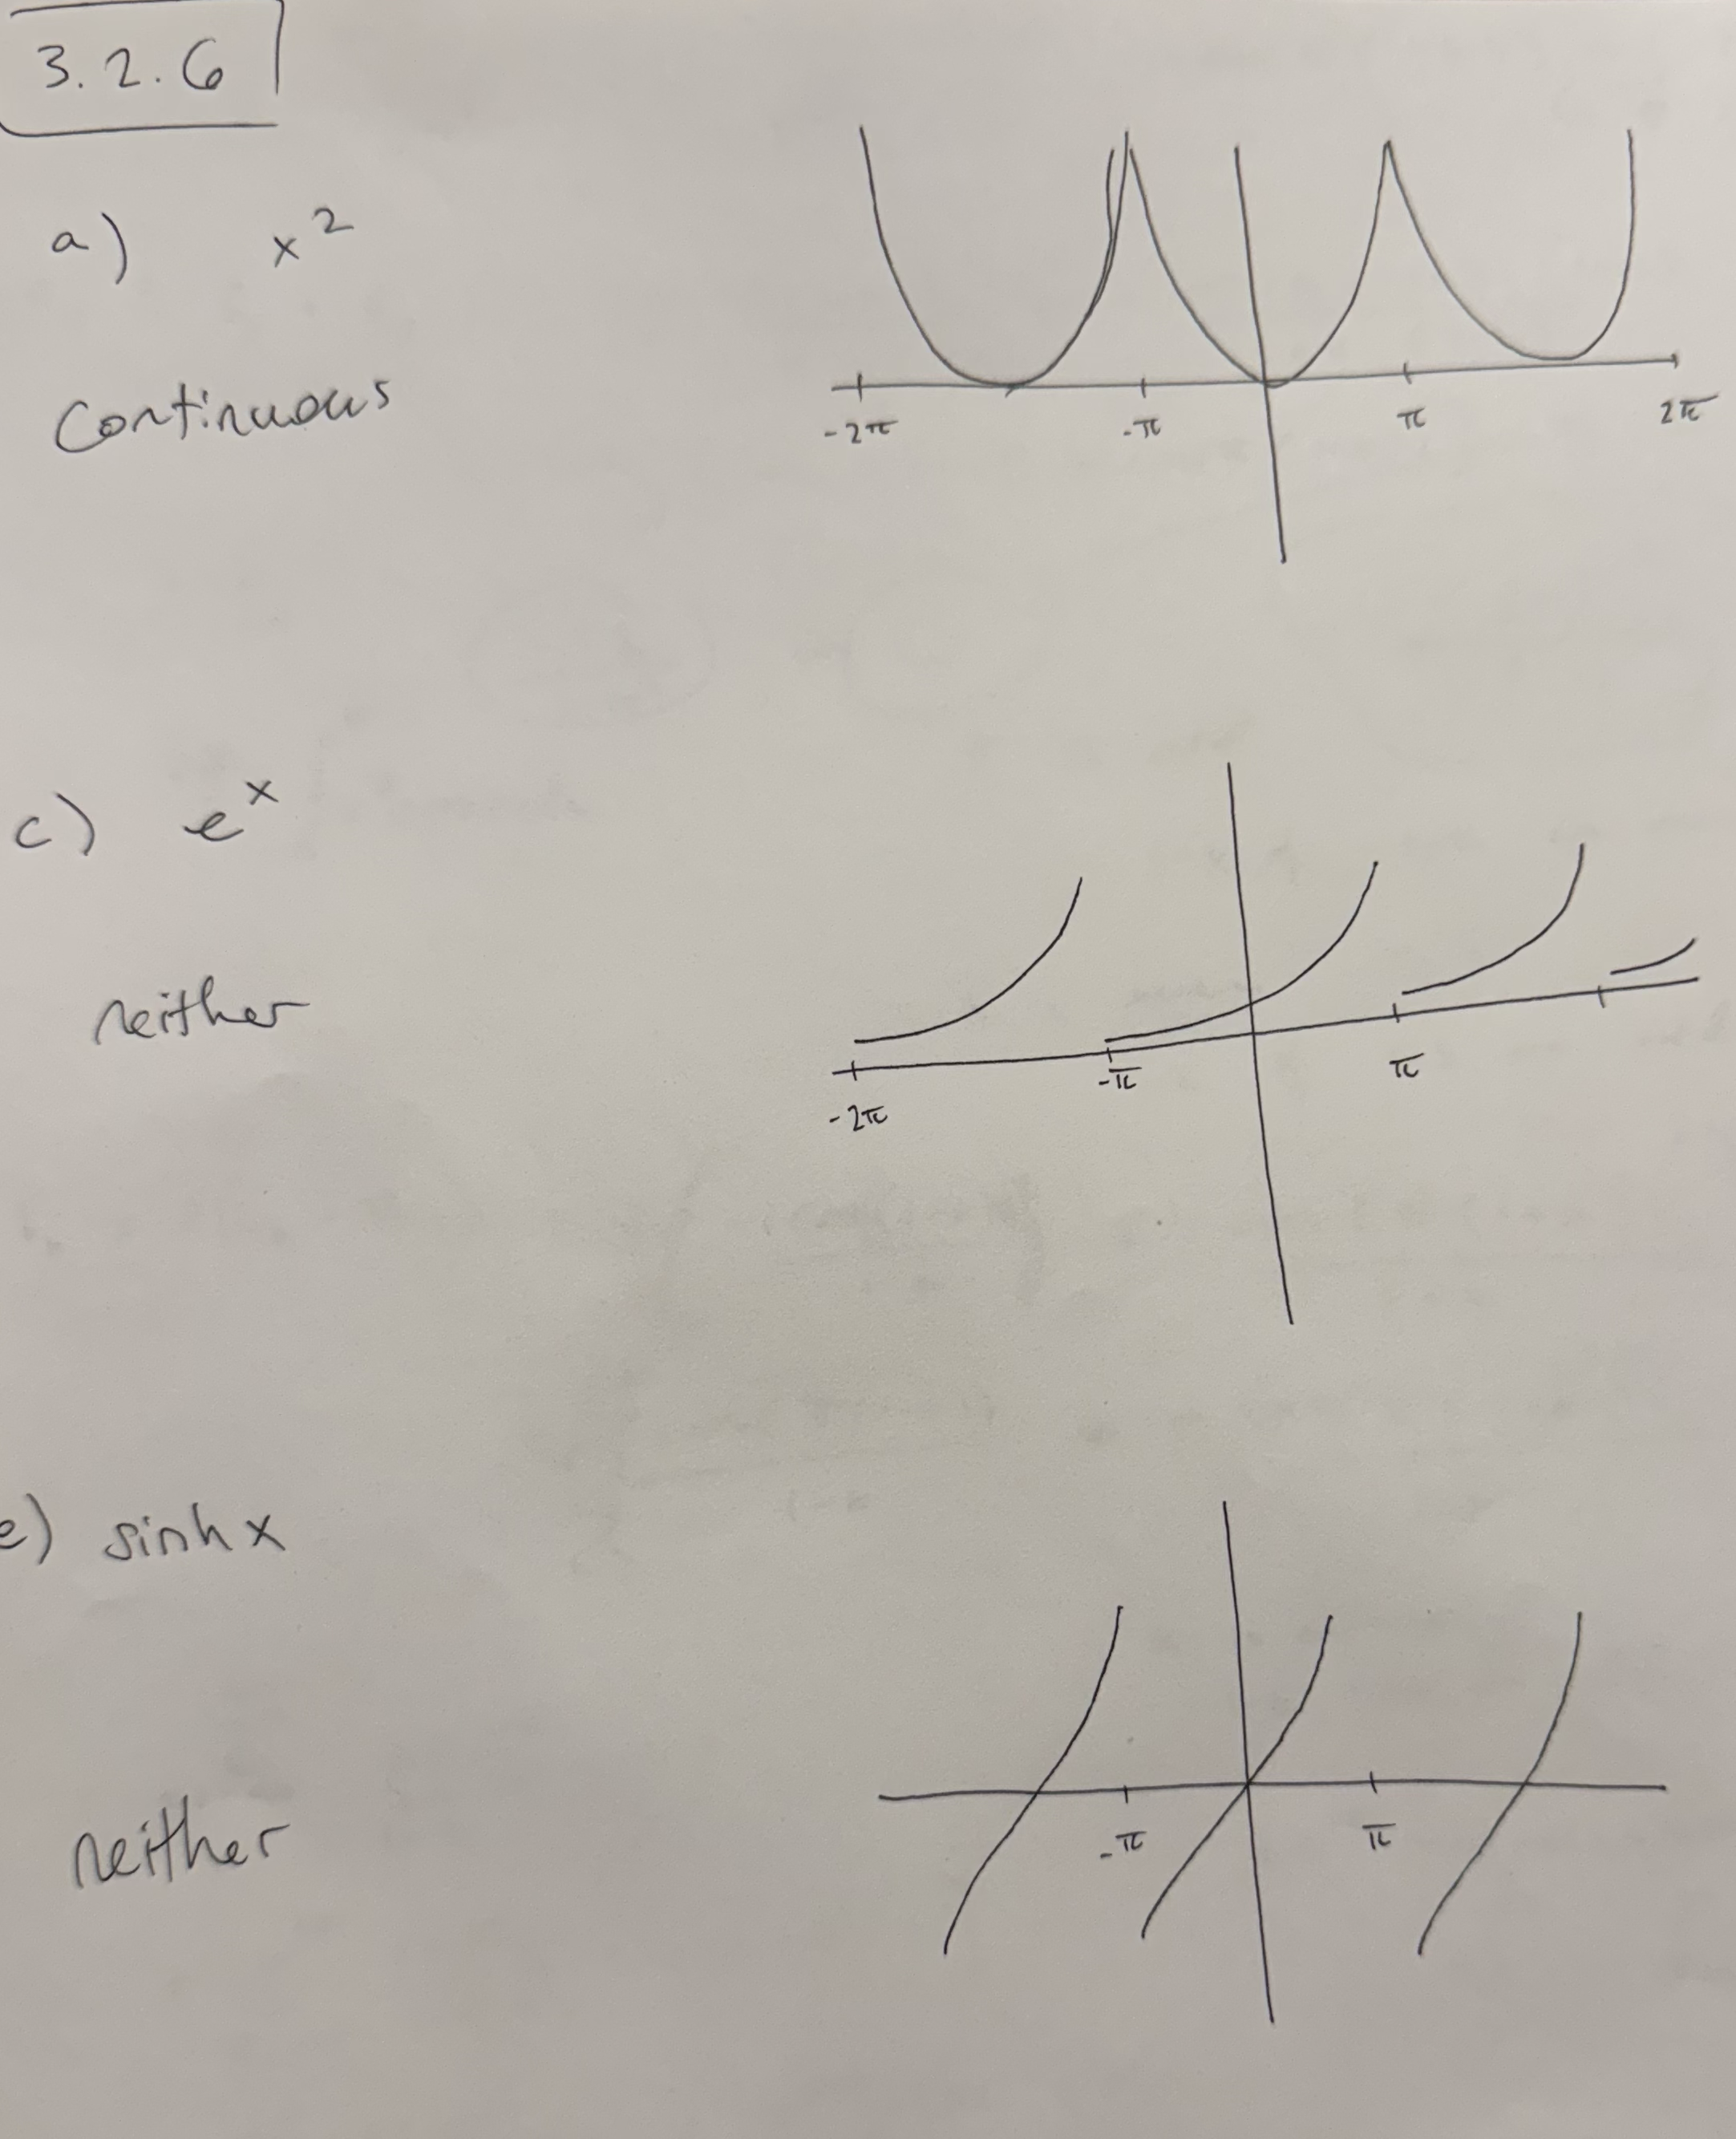
\includegraphics[width=.55\textwidth]{pdes_hw_03.png}
 	\caption{A sketch of the various $2\pi$ periodic extensions of the requested functions. }\label{fig:f1}
\end{figure}
\qed \\

\newpage


\item Olver: 3.3.2 and 3.3.3 \\
\begin{itemize}
\item 3.3.2 Find the Fourier series for the function $f(x) = x^3$.
If you differentiate your series, do you recover the Fourier series for $f^\prime(x) = 3x^2$?
If not, explain why not. \\

\noindent
\textit{Solution:} \\
We begin by calculating the coefficients $a_k$ and $b_k$
We first have,
$$
a_k = \langle x^3, \cos kx \rangle = \frac 1 \pi \int_{-\pi}^\pi x^3 \cos kx dx
$$
which leads us to use integration by parts where $u = x^3$, $dv = \cos kx dx$.
Notice we are going to need to do this iteratively where $u$ is always set to the polynomial part of the integrand and $dv$ is always the trigonometric part.
Therefore,
\begin{align*}
\frac 1 \pi \int_{-\pi}^\pi x^3 \cos kx dx
	&= \frac 1 \pi\left[ \left. x^3 \frac {\sin k x} k \right|_{-\pi}^\pi - \int_{-\pi}^\pi 3 x^2 \frac {\sin kx} k dx \right] \\
	&= \frac 1 \pi\left[
		\left. x^3 \frac {\sin k x} k \right|_{-\pi}^\pi
		+ \Bigg( \left. 3x^2 \frac {\cos k x} {k^2} \right|_{-\pi}^\pi - \int_{-\pi}^\pi 6 x \frac {\cos kx} {k^2} dx\Bigg)
	\right] \\
	&= \frac 1 \pi\left[
		\left. x^3 \frac {\sin k x} k \right|_{-\pi}^\pi
		+ \Bigg(
			\left. 3x^2 \frac {\cos k x} {k^2} \right|_{-\pi}^\pi
			- \Big( \left. 6x \frac {\sin k x} {k^3} \right|_{-\pi}^\pi - \int_{-\pi}^\pi 6 \frac {\sin k x} {k^3} dx \Big)
		\Bigg)
	\right] \\
	&= \frac 1 \pi\left[
		\left. x^3 \frac {\sin k x} k \right|_{-\pi}^\pi
		+ \Bigg(
			\left. 3x^2 \frac {\cos k x} {k^2} \right|_{-\pi}^\pi
			- \Big( \left. 6x \frac {\sin k x} {k^3} \right|_{-\pi}^\pi + \left. 6 \frac {\cos k x} {k^4} \right|_{-\pi}^\pi \Big)
		\Bigg)
	\right] \\
	&= \frac 1 \pi \left[ \left.
		x^3 \frac {\sin k x} k + 3x^2 \frac {\cos k x} {k^2} - 6x \frac {\sin k x} {k^3} - 6 \frac {\cos k x} {k^4} \right|_{-\pi}^\pi
	\right] \\
	&= \frac 1 \pi \left[
		\Bigg( (\pi)^3 \frac {\sin k \pi} k + 3(\pi)^2 \frac {\cos k \pi} {k^2} - 6\pi \frac {\sin k \pi} {k^3} - 6 \frac {\cos k \pi} {k^4} \Bigg) \right. \\
		&\quad\quad- \left. \Bigg( (-\pi)^3 \frac {\sin (- k \pi) } k + 3(-\pi)^2 \frac {\cos (- k \pi)} {k^2} + 6\pi \frac {\sin (- k \pi)} {k^3} - 6 \frac {\cos (- k \pi)} {k^4} \Bigg)
	\right].
\end{align*}
Each of the $\sin$ terms are 0 and the $\cos$ terms of different signs end up canceling one another out.
Thus we have
\begin{align*}
&= \frac 1 \pi \left[
		3(\pi)^2 \frac {\cos k \pi} {k^2} - 6 \frac {\cos k \pi} {k^4} - 3(\pi)^2 \frac {\cos (k \pi)} {k^2} + 6 \frac {\cos (k \pi)} {k^4}
	\right] = 0
\end{align*}
Which checks out since $x^3$ is an odd function, therefore it's Fourier series is going to be solely comprised of the $b_k$ and $\sin$ terms.
Calculating $b_k$ using repeated integration by parts we have
\begin{align*}
\frac 1 \pi \int_{-\pi}^\pi x^3 \sin kx dx
	&= \frac 1 \pi\left[ - \left. x^3 \frac {\cos k x} k \right|_{-\pi}^\pi + \int_{-\pi}^\pi 3 x^2 \frac {\cos kx} k dx \right] \\
	&= \frac 1 \pi\left[
		- \left. x^3 \frac {\cos k x} k \right|_{-\pi}^\pi
		+ \Bigg( \left. 3x^2 \frac {\sin k x} {k^2} \right|_{-\pi}^\pi - \int_{-\pi}^\pi 6 x \frac {\sin kx} {k^2} dx\Bigg)
	\right] \\
	&= \frac 1 \pi\left[
		- \left. x^3 \frac {\cos k x} k \right|_{-\pi}^\pi
		+ \Bigg(
			\left. 3x^2 \frac {\sin k x} {k^2} \right|_{-\pi}^\pi
			+ \Big( \left. 6x \frac {\cos k x} {k^3} \right|_{-\pi}^\pi - \int_{-\pi}^\pi 6 \frac {\cos k x} {k^3} dx \Big)
		\Bigg)
	\right] \\
	&= \frac 1 \pi\left[
		- \left. x^3 \frac {\cos k x} k \right|_{-\pi}^\pi
		+ \Bigg(
			\left. 3x^2 \frac {\sin k x} {k^2} \right|_{-\pi}^\pi
			+ \Big( \left. 6x \frac {\cos k x} {k^3} \right|_{-\pi}^\pi - \left. 6 \frac {\sin k x} {k^4} \right|_{-\pi}^\pi \Big)
		\Bigg)
	\right] \\
	&= \frac 1 \pi \left[ \left.
		- x^3 \frac {\cos k x} k + 3x^2 \frac {\sin k x} {k^2} + 6x \frac {\cos k x} {k^3} - 6 \frac {\sin k x} {k^4} \right|_{-\pi}^\pi
	\right] \\
	&= \frac 1 \pi \left[
		\Bigg( - (\pi)^3 \frac {\cos k \pi} k + 3(\pi)^2 \frac {\sin k \pi} {k^2} + 6\pi \frac {\cos k \pi} {k^3} - 6 \frac {\sin k \pi} {k^4} \Bigg) \right. \\
		&\quad\quad - \left. \Bigg( - (- \pi)^3 \frac {\cos (- k \pi)} k + 3(- \pi)^2 \frac {\sin (- k \pi)} {k^2} - 6\pi \frac {\cos (- k \pi)} {k^3} - 6 \frac {\sin (- k \pi)} {k^4} \Bigg)
	\right].
\end{align*}
Once more, we utilize the fact that the $\sin$ terms are all 0, and thus we have
\begin{align*}
&= \frac 1 \pi \left[ - \pi^3 \frac {\cos k \pi} k + 6\pi \frac {\cos k \pi} {k^3} - \pi^3 \frac {\cos (k \pi)} k + 6\pi \frac {\cos (- k \pi)} {k^3} \right] \\
&= \frac 1 \pi \left[ - 2 \pi^3 \frac {\cos k \pi} k + 12\pi \frac {\cos k \pi} {k^3} \right] \\
&= - 2 \pi^2 \frac {\cos k \pi} k + 12 \frac {\cos k \pi} {k^3} \\
&= \cos k \pi \left( \frac{12}{k^3} - \frac {2 \pi^2} k \right)  \\
&= (-1)^k \left( \frac{12}{k^3} - \frac {2 \pi^2} k \right).
\end{align*}
Therefore, the Fourier series of $x^3$ is
$$
x^3 \sim \sum_{k=1}^{\infty} (-1)^k \left( \frac{12}{k^3} - \frac {2 \pi^2} k \right) \sin k x.
$$
Now we are interested in seeing if the derivative of this series is the same as the Fourier series for the derivative of $x^3$.
\begin{align*}
\frac d {dx} \left [ \sum_{k=1}^{\infty} (-1)^k \left( \frac{12}{k^3} - \frac {2 \pi^2} k \right) \sin k x \right]
&=  \sum_{k=1}^{\infty} \frac d {dx} \left [ (-1)^k \left( \frac{12}{k^3} - \frac {2 \pi^2} k \right) \sin k x \right] \\
&=  \sum_{k=1}^{\infty} (-1)^k \left( \frac{12}{k^3} - \frac {2 \pi^2} k \right) \cos k x 
\end{align*}
This does not match the Fourier coefficient for $2x^3$ we computed manually. \\
\qed \\
\newpage

\item 3.3.3 Repeat exercise 3.3.2 but starting with $f(x) = x^4$. \\
\noindent
\textit{Solution:} \\
Notice, $x^4$ is an even function therefore we will forgo calculating the $b_k$ which will all be 0.
Instead we calculate the $a_k$ coeffs
\begin{align*}
a_k = \langle x^4, \cos kx \rangle &= \frac 1 \pi \int_{-\pi}^\pi x^4 \cos kx dx \\
	&= \frac 1 \pi\left[ \left. x^4 \frac {\sin k x} k \right|_{-\pi}^\pi - \int_{-\pi}^\pi 4 x^3 \frac {\sin kx} k dx \right] \\
	&= \frac 1 \pi\left[
		\left. x^4 \frac {\sin k x} k \right|_{-\pi}^\pi
		+ \Bigg( \left. 4x^3 \frac {\cos k x} {k^2} \right|_{-\pi}^\pi - \int_{-\pi}^\pi 12 x^2 \frac {\cos kx} {k^2} dx\Bigg)
	\right] \\
	&= \frac 1 \pi\left[
		\left. x^4 \frac {\sin k x} k \right|_{-\pi}^\pi
		+ \Bigg(
			\left. 4x^3 \frac {\cos k x} {k^2} \right|_{-\pi}^\pi
			- \Big( \left. 12x^2 \frac {\sin k x} {k^3} \right|_{-\pi}^\pi - \int_{-\pi}^\pi 24x \frac {\sin k x} {k^3} dx \Big)
		\Bigg)
	\right] \\
	&= \frac 1 \pi\left[
		\left. x^4 \frac {\sin k x} k \right|_{-\pi}^\pi
		+ \Bigg(
			\left. 4x^3 \frac {\cos k x} {k^2} \right|_{-\pi}^\pi
			- \Big( \left. 12x^2 \frac {\sin k x} {k^3} \right|_{-\pi}^\pi
				+ \big(
					\left. 24x \frac {\cos k x} {k^4} \right|_{-\pi}^\pi
					- \int_{-\pi}^\pi 24 \frac {\cos k x} {k^4} dx
				\big)
			\Big)
		\Bigg)
	\right] \\
	&= \frac 1 \pi \left[ \left.
		x^4 \frac {\sin k x} k + 4x^3 \frac {\cos k x} {k^2} - 12x^2 \frac {\sin k x} {k^3} - 24x \frac {\cos k x} {k^4} + 24 \frac {\sin k x} {k^5} \right|_{-\pi}^\pi 
	\right] \\
	&= \frac 1 \pi \left[
		\Bigg( (\pi)^4 \frac {\sin k \pi} k + 4(\pi)^3 \frac {\cos k \pi} {k^2} - 12\pi^2 \frac {\sin k \pi} {k^3} - 24 \pi \frac {\cos k \pi} {k^4} + 24 \frac {\sin k \pi} {k^5} \Bigg) \right. \\
		&\quad\quad - \left.\Bigg( (- \pi)^4 \frac {\sin (- k \pi)} k + 4(- \pi)^3 \frac {\cos (- k \pi)} {k^2} - 12(-\pi)^2 \frac {\sin (- k \pi)} {k^3} + 24 \pi \frac {\cos (- k \pi)} {k^4} + 24 \frac {\sin (- k \pi)} {k^5} \Bigg)
	\right]
\end{align*}
Once, again the $\sin$ terms are 0 but the $\cos$ terms won't cancel since they switch signs with odd power coefficients this time
\begin{align*}
&= \frac 1 \pi \left[
		4(\pi)^3 \frac {\cos k \pi} {k^2} - 24 \pi \frac {\cos k \pi} {k^4} - \Bigg( 4(- \pi)^3 \frac {\cos (- k \pi)} {k^2} + 24 \pi \frac {\cos (- k \pi)} {k^4} \Bigg)
	\right] \\
&= \frac 1 \pi \left[ 4(\pi)^3 \frac {\cos k \pi} {k^2} - 24 \pi \frac {\cos k \pi} {k^4} + 4(\pi)^3 \frac {\cos (k \pi)} {k^2} - 24 \pi \frac {\cos (k \pi)} {k^4} \right] \\
&= \cos k \pi \left( \frac {8\pi^2} {k^2} - \frac {48} {k^4} \right) \\
&= (-1)^k \left( \frac {8\pi^2} {k^2} - \frac {48} {k^4} \right). 
\end{align*}
Therefore, the Fourier series of $x^4$ is
$$
x^4 \sim \sum_{k=1}^{\infty} (-1)^k \left( \frac {8\pi^2} {k^2} - \frac {48} {k^4} \right) \cos k x.
$$
Similar to part 1, we have
\begin{align*}
\frac d {dx} \left[ \sum_{k=1}^{\infty} (-1)^k \left( \frac {8\pi^2} {k^2} - \frac {48} {k^4} \right) \cos k x \right] 
	&= \sum_{k=1}^{\infty} \frac d {dx} \left [ (-1)^k \left( \frac {8\pi^2} {k^2} - \frac {48} {k^4} \right) \cos k x \right] \\
	&= \sum_{k=1}^{\infty} (-1)^{k + 1} \left( \frac {8\pi^2} {k^2} - \frac {48} {k^4} \right) \sin k x.
\end{align*}
Which once again does not have the right coefficients for $4x^3$. \\
\qed \\
\end{itemize}

\newpage


\item Olver: 3.2.55 \\
\begin{enumerate}
\item Find the complex Fourier series for $x\E^{\I x}$ \\

\noindent
\textit{Solution:} \\
First of all we define the complex Fourier series for a piecewise continuous real or complex function $f$ is the doubly infinite series
$$
f(x) \sim \sum_{k=-\infty}^{\infty} c_k \E^{\I k x}
$$
where the $c_k$ are given by
$$
c_k = \langle f, \E^{\I k x} \rangle = \frac 1 {2 \pi} \int_{-\pi}^{\pi} f(x) \E^{-\I k x} dx.
$$
Therefore, the bulk of our work here is to establish what the coefficients $c_k$ need to be.
In other words we need to calculate
\begin{align*}
c_k = \langle x\E^{\I x}, \E^{\I k x} \rangle
	&= \frac 1 {2 \pi} \int_{-\pi}^{\pi} x\E^{\I x} \E^{-\I k x} dx \\
	&= \frac 1 {2 \pi} \int_{-\pi}^{\pi} x\E^{\I x (1 - k)}dx.
\end{align*}
I believe integration by parts would be useful.
Let $u = x$ and let $dv = \E^{\I x (1 - k)}dx$ these then also give rise to $du = dx$ and $v = \frac 1 {\I(1 - k)} \E^{\I x (1 - k)}$, respectively.
Then we have
\begin{align*}
\int u dv &= uv - \int v du \\
\frac 1 {2 \pi} \int_{-\pi}^{\pi} x\E^{\I x (1 - k)}dx
	&= \frac 1 {2 \pi} \Bigg[ \left. \frac x {\I(1 - k)} \E^{\I x (1 - k)}\right|_{-\pi}^{\pi} - \int_{-\pi}^{\pi} \frac 1 {\I(1 - k)} \E^{\I x (1 - k)} dx \Bigg] \\
\end{align*}
Let's take the right hand piece by piece in order to keep the calculations clean.
First with the $uv$ term
\begin{align*}
uv &= \left. \frac x {\I(1 - k)} \E^{\I x (1 - k)}\right|_{-\pi}^{\pi} \\
	&= \frac \pi {\I(1 - k)} \E^{\I \pi (1 - k)} - \frac {(-\pi)} {\I(1 - k)} \E^{- \I \pi (1 - k)} \\
	&= \frac \pi {\I(1 - k)} \left( \E^{\I \pi (1 - k)} + \E^{- \I \pi (1 - k)} \right) \\
	&= \frac {2 \pi \cos (\pi (1 - k)) } {\I(1 - k)} \\
	&= - \frac {2 \pi \I \cos (\pi (1 - k)) } {1 - k}.
\end{align*}
Now we proceed with the integral on the right hand side
\begin{align*}
\int v du &= \int_{-\pi}^{\pi} \frac 1 {\I(1 - k)} \E^{\I x (1 - k)} dx \\
	&= \left. \frac 1 {(\I(1 - k))^2} \E^{\I x (1 - k)} \right|_{-\pi}^{\pi} \\
	&= \frac 1 {(\I(1 - k))^2} \E^{\I \pi (1 - k)} - \frac 1 {(\I(1 - k))^2} \E^{- \I \pi (1 - k)} \\
	&= \frac 1 {\I^2(1 - k)^2} \left(  \E^{\I \pi (1 - k)} - \E^{- \I \pi (1 - k)} \right) \\
	&= - \frac 1 {(1 - k)^2} \left(  2 \I \sin (\pi (1 - k)) \right) \\
	&= 0
\end{align*}
where the final equality holds due to the fact that $\sin(\pi (1 - k))$ is always 0 since $1 - k$ is an integer.
Using these in our initial IBP step we have
\begin{align*}
\frac 1 {2 \pi} \int_{-\pi}^{\pi} x\E^{\I x (1 - k)}dx
	&= \frac 1 {2 \pi} \Bigg[ \left. \frac x {\I(1 - k)} \E^{\I x (1 - k)}\right|_{-\pi}^{\pi} - \int_{-\pi}^{\pi} \frac 1 {\I(1 - k)} \E^{\I x (1 - k)} dx \Bigg] \\
	&= \frac 1 {2 \pi} \Bigg[ - \frac {2 \pi \I \cos (\pi (1 - k)) } {1 - k} \Bigg] \\
	&= - \frac {\I \cos (\pi (1 - k)) } {1 - k}.
\end{align*}
Notice, since $\cos(\ell \pi) = \begin{cases} 1, &\text{if $\ell$ is even} \\ -1, &\text{if $\ell$ is odd} \end{cases}$, therefore, when $k$ is odd $1 - k$ is even but if $k$ is even then $1 - k$ is odd.
Hence
\begin{align*}
- \frac {\I \cos (\pi (1 - k)) } {1 - k} &= - \frac {\I (-1)^{(1 - k)} } {1 - k} \\
	&= \frac {\I (-1)^{(2 - k)} } {1 - k} \\
	&= \frac {\I (-1)^{k} } {1 - k}
\end{align*}
Thus we have calculated the $c_k$ to be
$$
c_k = \frac {\I (-1)^{k} } {1 - k}
$$
and thus our Fourier series of the function $x \E^{\I x}$ is given by
$$
f(x) \sim \sum_{k=-\infty}^{\infty} \frac {\I (-1)^{k} } {1 - k} \E^{\I k x}
$$
\qed \\

\item Use your result to write down the real Fourier series for $x\cos x$ and $x \sin s$ \\
\noindent
\textit{Solution:} \\
Notice we can rewrite the previous Fourier series as
\begin{align*}
f(x) &\sim \sum_{k=-\infty}^{\infty} \frac {\I (-1)^{k} } {1 - k} \E^{\I k x} \\
x \E^{\I x} &\sim \sum_{k=-\infty}^{\infty} \frac {\I (-1)^{k} } {1 - k} \E^{\I k x} \\
x \cos x + \I x\sin x &\sim \sum_{k=-\infty}^{\infty} \Bigg[ \frac {\I (-1)^{k} } {1 - k} \cos kx - \frac { (-1)^{k} } {1 - k}\sin kx \Bigg].
\end{align*}
Pairing up the real and imaginary parts of this we get
$$
x \cos x \sim \sum_{k=-\infty}^{\infty}  \frac { (-1)^{k + 1} } {1 - k}\sin kx
$$
and
$$
x \sin x \sim \sum_{k=-\infty}^{\infty} \frac {(-1)^{k} } {1 - k} \cos kx.
$$
However, for the real Fourier series we want the indices to start at $k=1$ rather than $-\infty$.
Thus we have
\begin{align*}
\sum_{k=-\infty}^{\infty}  \frac { (-1)^{k + 1} } {1 - k}\sin kx
	&= \sum_{k=1}^{\infty}  \Bigg[ \frac { (-1)^{k + 1} } {1 - k}\sin kx + \frac { (-1)^{-k + 1} } {1 + k}\sin (-kx) \Bigg] \\
	&= \sum_{k=1}^{\infty}  \frac { (-1)^{k + 1} \Big( \sin kx (1 + k) - \sin kx (1 - k) \Big)} {1 - k^2} \\
	&= \sum_{k=1}^{\infty}  \frac { (-1)^{k + 1} 2 k \sin kx} {1 - k^2}
\end{align*}
However, we actually want to exclude $k= 1$ to avoid dividing by zero.
Also it is helpful to note that we have already removed $k = 0$ since $\sin 0 = 0$
Thus
$$
x \cos x \sim \sum_{k=2}^{\infty}  \frac { (-1)^{k + 1} 2 k \sin kx} {1 - k^2}.
$$
Finally for $x \sin x$ we have
\begin{align*}
\sum_{k=-\infty}^{\infty} \frac {(-1)^{k} } {1 - k} \cos kx
	&= 1 + \sum_{k=1}^{\infty} \Bigg( \frac {(-1)^{k} } {1 - k} \cos kx + \frac {(-1)^{-k} } {1 + k} \cos (- kx) \Bigg) \\
	&= 1 + \sum_{k=1}^{\infty} (-1)^{k} \cos kx \Bigg( \frac {1} {1 - k}  + \frac { 1 } {1 + k} \Bigg) \\
	&= 1 + \sum_{k=1}^{\infty} \frac {(-1)^{k} \cos kx } {1 - k^2}.
\end{align*}
And thus
$$
x \sin x \sim 1 + \sum_{k=1}^{\infty} \frac {(-1)^{k} \cos kx } {1 - k^2}.
$$
\textbf{TODO: revisit this and verify how to handle the $k=1$ case.}


\end{enumerate}

\newpage


\item Olver: 3.4.6 Write down formulas for the Fourier series of both even and odd functions on $[-\ell, \ell]$. \\

\noindent
\textit{Solution:} \\
When $f$ is even on $[-\ell, \ell]$ we have
$$
f(x) \sim \frac {a_0} 2 + \sum_{k=1}^{\infty} a_k \cos \left( \frac {k \pi x }{\ell} \right).
$$
Additionally, when $f$ is odd on $[-\ell, \ell]$ we have
$$
f(x) \sim + \sum_{k=1}^{\infty} b_k \sin \left( \frac {k \pi x }{\ell} \right).
$$
\qed \\

\newpage


\item Olver: 3.5.29 Let $f(x) \in L^2[a, b]$ be square integrable.
Which constant function $g(x) \equiv c$ best approximates $f$ in the least squares sense? \\

\noindent
\textit{Solution:} \\
In the least squares sense, we want to find $c$ which solves
$$
\min || f(x) - c||^2
$$
Given our norm for $L^2$ we have
\begin{align*}
\frac d {dc} || f(x) - c||^2 &= \frac d {dc} \left[ \left( \sqrt{ \langle f(x) - c, f(x) - c \rangle } \right)^2 \right] \\
	&= \frac d {dc} \left[ \int_a^b (f(x) - c)^2 dx \right] \\
	&= \frac d {dc} \left[ \int_a^b (f(x))^2 - 2cf(x) + c^2 dx \right] \\
	&= \frac d {dc} \left[ \int_a^b (f(x))^2 dx - \int_a^b 2cf(x) dx + \int_a^b c^2 dx \right] \\
	&= - \int_a^b 2f(x) dx + \int_a^b 2c dx.
\end{align*}
Setting this equal to zero and solving for $c$ we have
\begin{align*}
- \int_a^b 2f(x) dx + \int_a^b 2c dx &= 0 \\
c &= \frac {\int_a^b 2f(x) dx}{\int_a^b 2 dx} \\
c &= \frac {\int_a^b f(x) dx}{\int_a^b dx} \\
c &= \frac 1 {b - a} \int_a^b 2f(x) dx.
\end{align*}
Therefore, this value of $c$ for the constant function $g(x) \equiv c$ best approximates $f$ in teh least squares sense. \\
\qed \\

\newpage


\item Olver: 3.5.43 For each $n = 1, 2, ..., $ define the function
$$
f_n(x) = \begin{cases} 1, \quad &\frac k m \leq x \leq \frac {k + 1} m, \\ 0, \quad & \text{otherwise}\end{cases},
$$
where $n = \frac 1 2 m (m + 1) + k$ and $0 \leq k \leq m$.
Show first that $m, k$ are uniquely determined by $n$.
Then prove that, on the interval $[0, 1]$, the sequence $f_n(x)$ converges in norm to 0 but does not converge pointwise \textit{anywhere}! \\

\noindent
\textit{Solution:} \\
We begin by showing that $n$ uniquely determines $k$ and $m$.
First, notice
$$
n = \frac 1 2 m(m + 1) + k \implies 0 = \frac 1 2 m^2 + \frac 1 2 m + (k - n).
$$
Hence,
$$
m = \frac {-1/2 \pm \sqrt{\frac 1 4 - 2(k - n)} }{2 (1/2)} = -\frac 1 2 \pm \sqrt{\frac 1 4 - 2(k - n)}
$$
\textbf{TODO: Revisit...} \\

\noindent
Now we want to show that the sequence converges in norm to 0.
Thus we need to show
$$
\lim_{n \rightarrow \infty} ||f_n(x) - 0|| = 0.
$$
Without further ado,
\begin{align*}
\lim_{n \rightarrow \infty} ||f_n(x) - 0|| &= \lim_{n \rightarrow \infty} ||f_n(x)|| \\
	&= \lim_{n \rightarrow \infty} \sqrt{ \langle  f_n(x), f_n(x) \rangle} \\
	&= \lim_{n \rightarrow \infty} \sqrt{ \int_0^1  f_n(x)^2 dx } \\
	&= \lim_{n \rightarrow \infty} \sqrt{
		\int_0^{\frac k m }  f_n(x)^2 dx
		+ \int_{\frac k m }^{\frac {k + 1} m }  f_n(x)^2 dx 
		+ \int_{\frac {k + 1} m }^1  f_n(x)^2 dx} \\
	&= \lim_{n \rightarrow \infty} \sqrt{\int_{\frac k m }^{\frac {k + 1} m } dx } \\
	&= \lim_{n \rightarrow \infty} \sqrt{ \frac {k + 1} m - \frac k m } \\
	&= \lim_{n \rightarrow \infty} \frac 1 {\sqrt{m }} \rightarrow 0
\end{align*}
Where we know $m$ is going to infinity as $n$ goes to infinity since $n$ depends on $n$ and $k$.
Therefore, $f_n$ converges to 0 in norm.
However, we claim that it does not converge point wise \textit{anywhere}!
The definition of point wise convergence is states as follows for all $\epsilon > 0$ and every $x \in I$ there exists $N \in \mathbb N$ depending on $\epsilon$ and $x$ such that
$$
| v_n(x) - v_*(x)| < \epsilon
$$
for all $n \geq N$.
I think I should show this by way of contradiction. \\
\qed \\

\newpage

\item We consider the complex orthonormal basis
$$
\varphi_n = \frac 1 {\sqrt{2 \pi}} \E^{\I n x}
$$
where $n = 0, 1, -1, 2, -2, ...$.
Consider the function $f_a(x) = \E^{ax}$ with real number $a \neq 0$ and compute the Fourier coefficient
$$
\langle f_a, \varphi_n \rangle = \frac 1 {\sqrt{2 \pi}} \int_{-\pi}^{\pi} f_a(x) \E^{- \I n x} dx.
$$
Then prove the formula
$$
\sum_{n = 1}^\infty \frac {1}{a^2 + n^2} = \frac \pi {2a} \coth (\pi a)  - \frac 1 {2a^2}
$$
(Hint: Plancherel’s formula: the relation between $L^2$ norm of coefficients and $\langle f_a, f_a \rangle$.)
\\

\noindent
\textit{Solution:} \\
We begin by calculating the Fourier coefficient as requested
\begin{align*}
\langle f_a, \varphi_n \rangle &= \frac 1 {\sqrt{2 \pi}} \int_{-\pi}^{\pi} f_a(x) \E^{- \I n x} dx \\
	&= \frac 1 {\sqrt{2 \pi}} \int_{-\pi}^{\pi} \E^{ax} \E^{- \I n x} dx \\
	&= \frac 1 {\sqrt{2 \pi}} \int_{-\pi}^{\pi} \E^{(a - \I n) x} dx \\
	&= \frac 1 {\sqrt{2 \pi}} \Bigg( \left. \frac 1 {(a - \I n)} \E^{(a - \I n) x} \right|_{-\pi}^{\pi} \Bigg) \\
	&= \frac 1 {\sqrt{2 \pi}} \Bigg( \frac 1 {(a - \I n)} \E^{(a - \I n) \pi} - \frac 1 {(a - \I n)} \E^{- (a - \I n) \pi} \Bigg) \\
	&= \frac 1 {\sqrt{2 \pi}(a - \I n)} \big( \E^{(a - \I n) \pi} - \E^{- (a - \I n) \pi} \big) \\
	&= \frac 1 {\sqrt{2 \pi}(a - \I n)} \big( \E^{a\pi} \E^{- \I n \pi} - \E^{- a\pi} \E^{ \I n \pi} \big) \\
	&= \frac 1 {\sqrt{2 \pi}(a - \I n)} \Bigg( \E^{a\pi} \Big( \cos{n \pi} - \cancelto{0}{\I \sin n \pi} \Big) - \E^{- a\pi} \Big( \cos{n \pi} + \cancelto{0}{\I \sin n \pi} \Big) \Bigg) \\
	&= \frac {\cos{n \pi}} {\sqrt{2 \pi}(a - \I n)} \big( \E^{a\pi} - \E^{- a\pi} \big) \\
	&= \frac {2 (-1)^n \sinh a \pi} {\sqrt{2 \pi}(a - \I n)}.
\end{align*}
This is the requested coefficient.

\newpage
\noindent
Next, let's prove the formula provided using \textbf{Theorem 3.43} from Olver, which states
$$
||f||^2 = \sum_{k=1}^\infty |c_k|^2 = \sum_{k=1}^{\infty} \langle f, \varphi_n \rangle^2.
$$
Notice, we have already calcualted $c_k = \langle f, \varphi_n \rangle$, thus
\begin{align*}
\sum_{k=1}^{\infty} |c_k|^2
	&= \sum_{k=-\infty}^{\infty} \left| \frac {2 (-1)^n \sinh a \pi} {\sqrt{2 \pi}(a - \I n)} \right| ^2 \\
	&= \sum_{k=-\infty}^{\infty} \frac {4 \sinh^2 a \pi} {2 \pi |a - \I n|^2} \\
	&= \sum_{k=-\infty}^{\infty} \frac {4 \sinh^2 a \pi} {2 \pi |a - \I n|^2} \\
	&= \sum_{k=-\infty}^{\infty} \frac {2 \sinh^2 a \pi} { \pi(a^2 + n^2)} \\
	&= \frac {2 \sinh^2 a \pi} { \pi} \sum_{k=-\infty}^{\infty} \frac 1 {a^2 + n^2}
\end{align*}
On the other hand we can calculate
\begin{align*}
||f_a||^2 = \langle \E^a, \E^a \rangle = \int_{-\pi}^{\pi} \E^{2ax} dx
	= \frac 1 {2a} \left( \E^{2a\pi} - \E^{- 2a\pi} \right) 
	= \frac {\sinh 2a\pi} {a}
\end{align*}
Hence,
\begin{align*}
||f_a||^2 &= \sum_{k=1}^\infty |c_k|^2 \\
\frac {\sinh 2a\pi} {a} &= \frac {2 \sinh^2 a \pi} { \pi} \sum_{k=-\infty}^{\infty} \frac 1 {a^2 + n^2} \\
\frac { \pi} {2 \sinh^2 a \pi} \frac {\sinh 2a\pi} {a} &=\sum_{k=-\infty}^{\infty} \frac 1 {a^2 + n^2} \\
\frac { \pi}{2a} \frac {\sinh 2a\pi} {\sinh^2 a \pi} &=\sum_{k=-\infty}^{\infty} \frac 1 {a^2 + n^2}
\end{align*}
We now employ the trig identity $\sinh 2x = 2\sinh x \cosh x $, thus
\begin{align*}
\frac { \pi}{2a} \frac {\sinh 2a\pi} {\sinh^2 a \pi} &=\sum_{k=-\infty}^{\infty} \frac 1 {a^2 + n^2} \\
\frac { \pi}{2a} \frac {2 \cancel{\sinh a\pi} \cosh a\pi} {\sinh^{\cancel{2}^1} a \pi} &=\sum_{k=-\infty}^{\infty} \frac 1 {a^2 + n^2} \\
\frac { \pi}{2a} \frac {2 \cosh a\pi} {\sinh a \pi} &=\sum_{k=-\infty}^{\infty} \frac 1 {a^2 + n^2} \\
\frac { \pi}{a} \coth a\pi &= \sum_{k=-\infty}^{\infty} \frac 1 {a^2 + n^2} \\
\frac { \pi}{a} \coth a\pi &= \frac 1 {a^2} + \sum_{\underset{k \neq 0}{k = -\infty}}^{\infty} \frac 1 {a^2 + n^2} \\
\frac { \pi}{a} \coth a\pi &= \frac 1 {a^2} + 2\sum_{k = 1}^{\infty} \frac 1 {a^2 + n^2} \\
\frac { \pi}{2a} \coth a\pi - \frac 1 {2a^2} &=  \sum_{k = 1}^{\infty} \frac 1 {a^2 + n^2} \\
\end{align*}
as requested. \\
\qed \\

\end{enumerate}

\end{document}

%%% Local Variables:
%%% mode: latex
%%% TeX-master: t
%%% End:
